\chapter{Perfectly Matched Layer \label{chap:pml}}

%\setcounter{page}{1}

\renewcommand{\thefootnote}{\fnsymbol{footnote}}
\footnotetext[2]{Lecture notes by John Schneider.  {\tt
fdtd-pml.tex}}

\section{Introduction}

The perfectly matched layer (PML) is generally considered the
state-of-the-art for the termination of FDTD grids.  There are some
situations where specially designed ABC's can outperform a PML, but
this is very much the exception rather than the rule.  The theory
behind a PML is typically pertinent to the continuous world.  In the
continuous world the PML should indeed work ``perfectly'' (as its
name implies) for all incident angles and for all frequencies.
However, when a PML is implemented in the discretized world of FDTD,
there are always some imperfections (i.e., reflections) present.

There are several different PML formulations.  However, all PML's
essentially act as a lossy material.  The lossy material, or lossy
layer, is used to absorb the fields traveling away from the interior
of the grid.  The PML is anisotropic and constructed in such a way
that there is no loss in the direction tangential to the interface
between the lossless region and the PML (actually there can be loss in
the non-PML region too, but we will ignore that fact for the moment).
However, in the PML there is always loss in the direction normal to
the interface.

The PML was originally proposed by J.-P. B\'{e}renger in 1994.  In
that original work he split each field component into two separate
parts.  The actual field components were the sum of these two parts
but by splitting the field B\'{e}renger could create an (non-physical)
anisotropic medium with the necessary phase velocity and conductivity
to eliminate reflections at an interface between a PML and non-PML
region.  Since B\'{e}renger first paper, others have described PML's
using different approaches such as the complex coordinate-stretching
technique put forward by Chew and Weedon, also in 1994.

Arguably the best PML formulation today is the Convolutional-PML
(CPML).  CPML constructs the PML from an anisotropic, dispersive
material.  CPML does not require the fields to be split and can be
implemented in a relatively straightforward manner.  

Before considering CPML, it is instructive to first consider a simple
lossy layer.  Recall that a lossy layer provided an excellent
ABC for 1D grids.  However, a traditional lossy layer does not work in
higher dimensions where oblique incidence is possible.  We will
discuss this and show how the split-field PML fixes this problem.

\section{Lossy Layer, 1D}

A lossy layer was previously introduced in Sec.\ \ref{sec:loss}.  Here
we will revisit lossy material but initially focus of the continuous
world and time-harmonic fields.  For continuous, time-harmonic fields,
the governing curl equations can be written
\begin{eqnarray}
  \nabla\times\Hvec &=&
    j\omega\epsilon\Evec + \sigma\Evec \,=\,
    j\omega\left(\epsilon - j\frac{\sigma}{\omega}\right)\Evec \,=\,
    j\omega\teps\,\Evec, \\
  \nabla\times\Evec &=&
    -j\omega\mu\Hvec - \sigma_m\Hvec \,=\,
    -j\omega\left(\mu - j\frac{\sigma_m}{\omega}\right)\Hvec \,=\,
    -j\omega\tmu\Hvec,
\end{eqnarray}
where the complex permittivity and permeability are given by
\begin{eqnarray}
  \teps &=& \epsilon - j\frac{\sigma}{\omega}, \\
  \tmu &=& \mu - j\frac{\sigma_m}{\omega}.
\end{eqnarray}

For now, let us restrict consideration to a 1D field that is
$z$-polarized so that the electric field is given by
\begin{equation}
  \Evec = \unitvec{z} e^{-\gamma x} = \unitvec{z} E_z(x)
\end{equation}
where the propagation constant $\gamma$ is yet to be determined.
Given the electric field, the magnetic field is given by
\begin{equation}
  \Hvec = -\frac{1}{j\omega\tmu} \nabla\times\Evec
        = -\unitvec{y}\frac{\gamma}{j\omega\tmu} E_z(x).
\end{equation}
Thus the magnetic field only has a $y$ component, i.e.,
$\Hvec=\unitvec{y}H_y(x)$.

The characteristic impedance of the medium $\eta$ is the ratio of the
electric field to the magnetic field (actually, in this case, the
negative of that ratio).  Thus,
\begin{equation}
  \eta = -\frac{E_z(x)}{H_y(x)} = \frac{j\omega\tmu}{\gamma}.
  \label{eq:almostEta}
\end{equation}
Since $\gamma$ has not yet been determined, we have not actually
specified the characteristic impedance yet.  To determine $\gamma$ we
use the other curl equation where we solve for the electric field in
terms of the magnetic field we just obtained:
\begin{equation}
  \Evec = \frac{1}{j\omega\teps}\nabla\times\Hvec
        = \frac{1}{j\omega\teps}
          \frac{\gamma^2}{j\omega\tmu}e^{-\gamma x} \unitvec{z}.
  \label{eq:eEqualsE}
\end{equation}
However, we already know the electric field since we started with that
as a given, i.e., $\Evec = \exp(-\gamma x)\unitvec{z}$.  Thus, in
order for \refeq{eq:eEqualsE} to be true, we must have
\begin{equation}
  \frac{\gamma^2}{(j\omega)^2\tmu\teps} = 1,
\end{equation}
or, solving for $\gamma$ (and only keeping the positive root)
\begin{equation}
  \gamma = j\omega\sqrt{\tmu\teps}.
\end{equation}
Because $\tmu$ and $\teps$ are complex, $\gamma$ will be complex and
we write $\gamma=\alpha + j\beta$ where $\alpha$ is the attenuation
constant and $\beta$ is the phase constant (or wave number).

Returning to the characteristic impedance as given in
\refeq{eq:almostEta}, we can now write
\begin{equation}
  \eta = \frac{j\omega\tmu}{j\omega\sqrt{\tmu\teps}}
       = \sqrt{\frac{\tmu}{\teps}}.
\end{equation}
Alternatively, we can write
\begin{equation}
  \eta = \sqrt{\frac{\mu\left(1-j\frac{\sigma_m}{\omega\mu}\right)}
              {\epsilon\left(1-j\frac{\sigma}{\omega\epsilon}\right)}}.
\end{equation}

Let us now consider a $z$-polarized plane wave normally incident from
a lossless material to a lossy material.  There is a planar interface
between the two media at $x=0$.  The (known) incident field
is given by
\begin{equation}
  E_z^i = e^{-j\beta_1x} \qquad H_y^i = -\frac{1}{\eta_1} e^{-j\beta_1x}
\end{equation}
where $\beta_1=\omega\sqrt{\mu_1\epsilon_1}$.  The reflected field is
given by
\begin{equation}
  E_z^r = \Gamma e^{j\beta_1x} \qquad H_y^r = \frac{\Gamma}{\eta_1} e^{j\beta_1x}
\end{equation}
where the only unknown is the reflection coefficient $\Gamma$.  The
transmitted field is given by
\begin{equation}
  E_z^t = T e^{-\gamma_2x} \qquad H_y^t = -\frac{T}{\eta_2}
                                           e^{-\gamma_2 x}
\end{equation}
where the only unknown is the transmission coefficient $T$.

Both the electric field and the magnetic field are tangential to the
interface at $x=0$.  Thus, the boundary conditions dictate that the
sum of the incident and reflected field must equal the transmitted
field at $x=0$.  Matching the electric fields at the interface yields
\begin{equation}
  1+\Gamma = T.  \label{eq:matchingE1D}
\end{equation}
Matching the magnetic fields yields
\begin{equation}
  -\frac{1}{\eta_1} + \frac{\Gamma}{\eta_1} = -\frac{T}{\eta_2}
\end{equation}
or, rearranging slightly,
\begin{equation}
  1 - \Gamma = \frac{\eta_1}{\eta_2}T. \label{eq:matchingH1D}
\end{equation}
Adding \refeq{eq:matchingE1D} and \refeq{eq:matchingH1D} and
rearranging yields
\begin{equation}
  T = \frac{2\eta_2}{\eta_2+\eta_1}.
\end{equation}
Plugging this back into \refeq{eq:matchingE1D} yields
\begin{equation}
  \Gamma = \frac{\eta_2-\eta_1}{\eta_2+\eta_1}.
  \label{eq:pmlGamma1D}
\end{equation}

Consider the case where the media are related by
\begin{equation}
  \frac{\mu_2}{\epsilon_2} = \frac{\mu_1}{\epsilon_1} 
  \qquad \mbox{and} \qquad
  \frac{\sigma_m}{\mu_2} = \frac{\sigma}{\epsilon_2}.
\end{equation}
We will call these conditions the ``matching conditions.''  Under
these conditions the impedances equal: 
\begin{equation}
  \eta_2=\sqrt{\frac{\mu_2\left(1-j\frac{\sigma_m}{\omega\mu_2}\right)}
             {\epsilon_2\left(1-j\frac{\sigma}{\omega\epsilon_2}\right)}}
  = \sqrt{\frac{\mu_1\left(1-j\frac{\sigma}{\omega\epsilon_2}\right)}
             {\epsilon_1\left(1-j\frac{\sigma}{\omega\epsilon_2}\right)}}
  = \sqrt{\frac{\mu_1}{\epsilon_1}} = \eta_1.
\end{equation}
When the impedances are equal, from \refeq{eq:pmlGamma1D} we see that
the reflection coefficient must be zero (and the transmission
coefficient is unity).  We further note that this is true independent
of the frequency.

As we have seen previously, this type of lossy layer can be
implemented in an FDTD grid.  To minimize numeric artifacts it is best
to gradually increase the conductivity within the lossy region.  Any
field that makes it to the end of the grid will be reflected, but,
because of the loss, this reflected field can be greatly attenuated.
Furthermore, as the field propagates back through the lossy region
toward the lossless region, it is further attenuated.  Thus the
reflected field from this lossy region (and the termination of the
grid) can be made relatively inconsequential.

\section{Lossy Layer, 2D}

Since a lossy layer works so well in 1D and is so easy to implement,
it is natural to ask if it can be used in 2D.  The answer, we shall
see, is that a simple lossy layer cannot be matched to the lossless
region for obliquely traveling waves.

Consider a TM$^z$ field where the incident electric field is given by
\begin{eqnarray}
  \Evec^i &=& \unitvec{z} e^{-j\kvec_1\cdot\rvec}, \\
      &=& \unitvec{z} e^{-j\beta_1\cos(\theta_i)x -j\beta_1\sin(\theta_i)y}, \\
      &=& \unitvec{z} e^{-j\beta_{1x}x -j\beta_{1y}y}.
\end{eqnarray}
Knowing that the angle of incidence equals the angle of reflection
(owing to the required phase matching along the interface), the
reflected field is given by
\begin{equation}
  \Evec^r  = \unitvec{z} \Gamma e^{j\beta_{1x}x -j\beta_{1y}y}.
\end{equation}
Combining the incident and reflected field yields
\begin{equation}
  \Evec_1  = \unitvec{z} 
             \left( e^{-j\beta_{1x}x} + \Gamma e^{j\beta_{1x}x}\right)
            e^{-j\beta_{1y}y}
           = \unitvec{z} E_{1z}.
\end{equation}
The magnetic field in the first medium is given by
\begin{eqnarray}
  \Hvec_1 &=& -\frac{1}{j\omega\mu_1}\nabla\times\Evec_1, \\
    &=& \unitvec{x}\frac{\beta_{1y}}{\omega\mu_1}
      \left(e^{-j\beta_{1x}x} + \Gamma e^{\beta_{1x}x}\right)
      e^{-j\beta_{1y}y}
    + \unitvec{y}\frac{\beta_{1x}}{\omega\mu_1}
      \left(-e^{-j\beta_{1x}x} + \Gamma e^{\beta_{1x}x}\right)
      e^{-j\beta_{1y}y}.
\end{eqnarray}

The transmitted electric field is
\begin{eqnarray}
  \Evec^t &=& \unitvec{z} T e^{-\gammavec_2\cdot\rvec} \\
          &=& \unitvec{z} T e^{-\gamma_{2x}x - \gamma_{2y}y}, \\
	  &=& \unitvec{z} E^t_z.
\end{eqnarray}
Plugging this expression into Maxwell's equations (or, equivalently,
the wave equation) ultimately yields the constraint equation
\begin{equation}
  \gamma_{2x}^2 + \gamma_{2y}^2 = -\omega^2\tmu_2\teps_2.
  \label{eq:gammaConstraint}
\end{equation}
Owing to the boundary condition that the fields must match at the
interface, the propagation in the $y$ direction (i.e., tangential to
the boundary) must be the same in both media.  Thus,
$\gamma_{2y} = j\beta_{1y}$.  Plugging this into \refeq{eq:gammaConstraint}
and solving for $\gamma_{2x}$ yields
\begin{equation}
  \gamma_{2x} = \sqrt{\beta_{1y}^2 -\omega^2\tmu_2\teps_2} 
    = \alpha_{2x} + j\beta_{2x}.
\end{equation}
Note that when $\beta_{1y}=0$, i.e., there is no propagation in the $y$
direction and the field is normally incident on the interface, this
reduces to $\gamma_{2x} = j\omega\sqrt{\tmu_2\teps_2}$ which is what
we had for the 1D case.  On the other hand, when $\sigma=\sigma_m=0$
we obtain $\gamma_{2x} = j\left(\omega^2\mu_2\epsilon_2 -
\beta_{1y}^2\right)^{1/2}$ where the term in parentheses is purely real
(so that $\gamma_{2x}$ will either be purely real or purely
imaginary).  The transmitted magnetic field is given by
\begin{eqnarray}
  \Hvec^t &=& -\frac{1}{j\omega\tmu_2}\nabla\times\Evec^t, \\
    &=& \unitvec{x} \frac{\beta_{1y}}{\omega\tmu_2} E_z^t -
        \unitvec{y} \frac{\gamma_{2x}}{j\omega\tmu_2} E_z^t.
\end{eqnarray}

Enforcing the boundary condition on the electric field and the
$y$-component of the magnetic field at $x=0$ yields
\begin{eqnarray}
  1 + \Gamma &=& T, \label{eq:eMatchingOblique} \\
  \frac{\beta_{1x}}{\omega\mu_1}\left(-1+\Gamma\right) &=&
  -\frac{\gamma_{2x}}{j\omega\tmu_2} T,
\end{eqnarray}
or, rearranging the second equation, 
\begin{equation}
  1-\Gamma = \frac{\mu_1\gamma_{2x}}{j\tmu_2 \beta_{1x}} T.
 \label{eq:hMatchingOblique} 
\end{equation}
Adding \refeq{eq:eMatchingOblique}  and \refeq{eq:hMatchingOblique}
and rearranging  yields
\begin{equation}
  T = \frac{j\frac{2\tmu_2}{\gamma_{2x}}}
           {j\frac{\tmu_2}{\gamma_{2x}} + \frac{\mu_1}{\beta_{1x}}}.
\end{equation}
Using this in \refeq{eq:eMatchingOblique} yields the reflection
coefficient
\begin{equation}
  \Gamma = \frac{j\frac{\tmu_2}{\gamma_{2x}} - \frac{\mu_1}{\beta_{1x}}}
                {j\frac{\tmu_2}{\gamma_{2x}} + \frac{\mu_1}{\beta_{1x}}}.
\end{equation}

The reflection coefficient will be zero only if the terms in the
numerator cancel.  Let us consider these terms individually.
Additionally, let us enforce a more restrictive form of the matching
conditions where now $\mu_2=\mu_1$, $\epsilon_2=\epsilon_1$ and, as
before, $\sigma/\epsilon_2=\sigma_m/\mu_2$.  The first term in the
numerator can be written
\begin{eqnarray}
  j\frac{\tmu_2}{\gamma_{2x}} &=& 
    \frac{\tmu_2}{\sqrt{\omega^2\tmu_2\teps_2-\beta_{1y}^2}}, \\
  &=&
   \frac{\mu_1\left(1-j\frac{\sigma}{\omega\epsilon_1}\right)}
   {\sqrt{\omega^2\mu_1\epsilon_1\left(1-j\frac{\sigma}{\omega\epsilon_1}\right)^2-\beta_{1y}^2}}, \\
  &=&
  \frac{\mu_1}
  {\sqrt{\omega^2\mu_1\epsilon_1-\frac{\beta_{1y}^2}
                                      {\left(1-j\frac{\sigma}{\omega\epsilon_1}\right)^2}}}.
  \label{eq:lossGammaNum1}
\end{eqnarray}
The second term in the numerator of the reflection coefficient is
\begin{equation}
  \frac{\mu_1}{\beta_{1x}} =   
  \frac{\mu_1}{\sqrt{\omega^2\mu_1\epsilon_1-\beta_{1y}^2}}.
  \label{eq:lossGammaNum2}
\end{equation}
Clearly \refeq{eq:lossGammaNum1} and \refeq{eq:lossGammaNum2} are not
equal (unless we further require that $\sigma=0$, but then the lossy
layer is not lossy).  Thus, for oblique incidence, the numerator of
the reflection coefficient cannot be zero and there will always be
some reflection from this lossy medium.

\section{Split-Field Perfectly Matched Layer}

To obtain a perfect match between the lossless and lossy regions,
B\'{e}renger proposed a non-physical anisotropic material known as a
perfectly matched layer (PML).  In a PML there is no loss in the
direction tangential to the interface but there is loss normal to the
interface.

First, consider the governing equations for the components of the
magnetic fields for TM$^z$ polarization.  We have
\begin{eqnarray}
  j\omega\mu_2 H_y + \sigma_{mx} H_y &=& \frac{\partial E_z}{\partial x} \\
  j\omega\mu_2 H_x + \sigma_{my} H_x &=& -\frac{\partial E_z}{\partial y}
\end{eqnarray}
where $\sigma_{mx}$ and $\sigma_{my}$ are the magnetic conductivities
associated {\em not} with the $x$ and $y$ components of the magnetic
field, but rather with propagation in the $x$ or $y$ direction.  (Note
that for 1D propagation in the $x$ direction the non-zero fields are
$H_y$ and $E_z$ while for 1D propagation in the $y$ direction they are
$H_x$ and $E_z$.)

For the electric field the governing equation is
\begin{equation}
  j\omega\epsilon_2 E_z + \sigma E_z = 
  \frac{\partial H_y}{\partial x} - \frac{\partial H_x}{\partial y}
  \label{eq:pmlEBeforeSplit}
\end{equation}
Here there is a single conductivity and no possibility to have explicitly
anisotropic behavior of the electrical conductivity.  Thus, it would
still be impossible to match the lossy region to the lossless one.

B\'{e}renger's fix was to split the electric field into two
(non-physical) components.  To get the ``actual'' field, we merely sum
these components.  Thus we write
\begin{equation}
  E_z = E_{zx} + E_{zy}
\end{equation}
These components are governed by 
\begin{eqnarray}
  j\omega\epsilon_2 E_{zx} + \sigma_x E_{zx} &=& \frac{\partial H_y}{\partial x},  \\
  j\omega\epsilon_2 E_{zy} + \sigma_y E_{zy} &=& -\frac{\partial H_x}{\partial y}.
\end{eqnarray}
Note that there are now two electrical conductivities: $\sigma_x$ and
$\sigma_y$.  If we set $\sigma_x = \sigma_y = \sigma$ and add these
two equations together, we recover the original equation
\refeq{eq:pmlEBeforeSplit}.  Further note that if
$\sigma_y=\sigma_{my}=0$ but $\sigma_x\neq 0$ and $\sigma_{mx}\neq 0$,
then a wave with components $H_x$ and $E_{zy}$ would not attenuate
while a wave with components $H_y$ and $E_{zx}$ would attenuate.

Let us define the terms $S_w$ and $S_{mw}$ as
\begin{eqnarray}
   S_w &=& 1 + \frac{\sigma_w}{j\omega\epsilon_2} \\
   S_{mw} &=& 1 + \frac{\sigma_{mw}}{j\omega\mu_2}
\end{eqnarray}
where $w$ is either $x$ or $y$.  We can then write the governing
equations as 
\begin{eqnarray}
  j\omega\epsilon_2 S_x E_{zx} &=& \frac{\partial H_y}{\partial x}, 
    \label{eq:ezxSplit} \\
  j\omega\epsilon_2 S_y E_{zy} &=& -\frac{\partial H_x}{\partial y},
    \label{eq:ezySplit} \\
  j\omega\mu_2 S_{mx} H_y &=& 
    \frac{\partial}{\partial x} \left(E_{zx}+E_{zy}\right),
    \label{eq:hySplit} \\
  j\omega\mu_2 S_{my} H_x &=& 
    -\frac{\partial}{\partial y} \left(E_{zx}+E_{zy}\right).
    \label{eq:hxSplit}
\end{eqnarray}
Taking the partial of \refeq{eq:hySplit} with respect to $x$ and then
substituting in the left-hand side of \refeq{eq:ezxSplit} yields
\begin{equation}
  -\omega^2\mu_2\epsilon_2 S_x S_{mx} E_{zx} =
    \frac{\partial^2}{\partial x^2} \left(E_{zx}+E_{zy}\right).
\end{equation}
Taking the partial of \refeq{eq:hxSplit} with respect to $y$ and then
substituting in the left-hand side of \refeq{eq:ezySplit} yields
\begin{equation}
  -\omega^2\mu_2\epsilon_2 S_y S_{my} E_{zy} =
    \frac{\partial^2}{\partial y^2} \left(E_{zx}+E_{zy}\right).
\end{equation}
Adding these two expressions together after dividing by the $S$ terms
yields
\begin{equation}
  -\omega^2\mu_2\epsilon_2 \left(E_{zx} + E_{zy}\right) =
  \left(\frac{1}{S_{mx}S_x} \frac{\partial^2}{\partial x^2} +
        \frac{1}{S_{my}S_y}  \frac{\partial^2}{\partial y^2}\right)
  \left(E_{zx} + E_{zy}\right)
\end{equation}
or, after rearranging and recalling that $E_{zx} + E_{zy} = E_z$,
\begin{equation}
  \left(\frac{1}{S_{mx}S_x} \frac{\partial^2}{\partial x^2} +
        \frac{1}{S_{my}S_y}  \frac{\partial^2}{\partial y^2} +
        \omega^2\mu_2\epsilon_2
  \right) E_z = 0.
\end{equation}
To satisfy this equation the transmitted field in the PML region would
be given by
\begin{equation}
  E_z^t = T e^{-j\sqrt{S_{mx}S_x}\beta_{2x} x -j\sqrt{S_{my}S_y}\beta_{2y} y}
\end{equation}
where we must also have
\begin{equation}
  \beta_{2x}^2 + \beta_{2y}^2 = \omega^2 \mu_2\epsilon_2.
\end{equation}

Using \refeq{eq:hySplit}, the $y$ component of the magnetic field in
the PML is given by
\begin{eqnarray}
  H_y^t &=& \frac{1}{j\omega\mu_2 S_{mx}}
          \frac{\partial E_z^t}{\partial x} \\
        &=& -\frac{\sqrt{S_{mx}S_x}\beta_{2x}}{\omega\mu_2 S_{mx}} E_z^t, \\
        &=& -\frac{\beta_{2x}}{\omega\mu_2}
             \sqrt{\frac{S_x}{S_{mx}}} E_z^t.
\end{eqnarray}
As always, the tangential fields must match at the interface.
Matching the electric fields again yields
\refeq{eq:eMatchingOblique}.  Matching the $y$ component of the
magnetic fields yields
\begin{equation}
  1 - \Gamma = \frac{\mu_1 \beta_{2x}}{\mu_2 \beta_{1x}}
               \sqrt{\frac{S_x}{S_{mx}}} T.
\end{equation}
Using this and \refeq{eq:eMatchingOblique} to solve for the
transmission and reflection coefficients yields
\begin{eqnarray}
  T &=& \frac{2\frac{\beta_{1x}}{\mu_1}}
           {\frac{\beta_{1x}}{\mu_1} + \frac{\beta_{2x}}{\mu_2}
               \sqrt{\frac{S_x}{S_{mx}}}}, \\
  \Gamma &=&  \frac{\frac{\beta_{1x}}{\mu_1} - \frac{\beta_{2x}}{\mu_2}
               \sqrt{\frac{S_x}{S_{mx}}}}
           {\frac{\beta_{1x}}{\mu_1} + \frac{\beta_{2x}}{\mu_2}
               \sqrt{\frac{S_x}{S_{mx}}}}.
  \label{eq:gPml2D}
\end{eqnarray}

It is now possible to match the PML to the non-PML region so that
$\Gamma$ is zero.  We begin by setting $\mu_2=\mu_1$ and
$\epsilon_2=\epsilon_1$.  Thus we have
$\omega^2\mu_2\epsilon_2=\omega^2\mu_1\epsilon_1$ and
\begin{eqnarray}
  \beta_{2x} &=& \left(\omega^2\mu_2\epsilon_2 - \beta_{2y}^2\right)^{1/2}, \\
         &=& \left(\omega^2\mu_1\epsilon_1 - \beta_{2y}^2\right)^{1/2}.
  \label{eq:k2xPml}
\end{eqnarray}
Recall that within the PML the propagation in the $y$ direction is not
given by $\beta_{2y}$ but rather by $\sqrt{S_y S_{my}}\beta_{2y}$.
Phase matching along the interface requires that
\begin{equation}
  \sqrt{S_y S_{my}}\beta_{2y} = \beta_{1y}.
\end{equation}
If we let $S_y = S_{my} = 1$, which can be realized by setting
$\sigma_y=\sigma_{my}=0$, then the phase matching condition reduces to
\begin{equation}
  \beta_{2y} = \beta_{1y}.
\end{equation}
Then, from \refeq{eq:k2xPml}, we have
\begin{eqnarray}
  \beta_{2x} &=& \left(\omega^2\mu_1\epsilon_1 - \beta_{1y}^2\right)^{1/2},\\
         &=&  \beta_{1x}.
\end{eqnarray}
Returning to \refeq{eq:gPml2D}, we now have 
\begin{eqnarray}
  \Gamma &=&  \frac{\frac{\beta_{1x}}{\mu_1} - \frac{\beta_{1x}}{\mu_1}
               \sqrt{\frac{S_x}{S_{mx}}}}
           {\frac{\beta_{1x}}{\mu_1} + \frac{\beta_{1x}}{\mu_1}
               \sqrt{\frac{S_x}{S_{mx}}}}, \\
   &=& \frac{1 - \sqrt{\frac{S_x}{S_{mx}}}}
            {1 + \sqrt{\frac{S_x}{S_{mx}}}}.
\end{eqnarray}
The last remaining requirement to achieve a perfect match is to have
$S_x=S_{mx}$.  This can be realized by having $\sigma_x/\epsilon_2 =
\sigma_{mx}/\mu_2$.  

To summarize, the complete set of matching
conditions for a constant-$x$ interface are
\begin{eqnarray}
  \epsilon_2 &=& \epsilon_1 \\
  \mu_2 &=& \mu_1 \\
  \sigma_y &=& \sigma_{my} \,=\, 0 \\
  \frac{\sigma_x}{\epsilon_2} &=& \frac{\sigma_{mx}}{\mu_2}.
\end{eqnarray}
Under these conditions propagation in the PML is governed by
\begin{eqnarray}
  e^{-j S_x \beta_{1x} x - j \beta_{1y} y} &=& 
  \exp\!\left(-j \left(1 + \frac{\sigma}{j\omega\epsilon_1}\right) \beta_{1x} x
   - j \beta_{1y} y\right), \\
 &=&  \exp\!\left(-\frac{\beta_{1x}\sigma}{\omega\epsilon_1}x\right)
  e^{-j\beta_{1x} x - j \beta_{1y} y}.
\end{eqnarray}
This shows that there is exponential decay in the $x$ direction but
otherwise the phase propagates in exactly the same way as it does in
the non-PML region.

\section{Un-Split PML}

In the previous section we had $S_w$ and $S_{mw}$ where $w\in\{x,y\}$.
However, once the matching condition has been applied, i.e.,
$\sigma_w/\epsilon_2 = \sigma_{mw}/\mu_2$, then we have $S_w=S_{mw}$.
Hence we will drop the $m$ from the subscript.  Additionally, with the
understanding that we are talking about the PML region, we will drop
the subscript $2$ from the material constants.  We thus write
\begin{equation}
  S_w = 1 + \frac{\sigma_w}{j\omega\epsilon}.
\end{equation}
The conductivity in the PML is not dictated by underlying parameters
in the physical space being modeled.  Rather, this conductivity is set
so as to minimize the reflections from the termination of the grid.
In that sense $\sigma_w$ is somewhat arbitrary.  Therefore let us
normalize the conductivity by the relative permittivity that pertains
at that particular location, i.e., 
\begin{equation}
  S_w = 1 + \frac{\sigma'_w}{j\omega\epsilon_0}
\end{equation}
where $\sigma'_w = \sigma_w/\epsilon_r$.  However, since the
conductivity has not yet been specified, we drop the prime and merely
write 
\begin{equation}
  S_w = 1 + \frac{\sigma_w}{j\omega\epsilon_0}
\end{equation}

Note that there could potentially be a problem with $S_w$ when the
frequency goes to zero.  In practice, in the curl equations this term
is also multiplied by $\omega$ and in that sense this is not a major
problem.  However, if we want to move these $S_w$ terms around, low
frequencies may cause problems.  To fix this, we add an additional
factor to ensure that $S_w$ remains finite as the frequency goes to
zero.

We can further generalize $S_w$ by allowing the leading term to take
on values other than unity.  This is effectively equivalent to
allowing the relative permittivity in the PML to change.  The general
expression for $S_w$ we will use is
\begin{equation}
  S_w = \kappa_w + \frac{\sigma_w}{a_w + j\omega\epsilon_0}.
\end{equation}
For the sake of considering 3D problems we also assume $w\in\{x,y,z\}$.

Dividing by the $S$ terms, the governing equations for TM$^z$
polarization are
\begin{eqnarray}
  j\omega\epsilon E_{zx} &=& 
    \frac{1}{S_x}\frac{\partial H_y}{\partial x}, \\
  j\omega\epsilon E_{zy} &=& 
    -\frac{1}{S_y}\frac{\partial H_x}{\partial y}, \\
  j\omega\mu H_y &=& 
    \frac{1}{S_x}\frac{\partial E_z}{\partial x},\\
  j\omega\mu H_x &=& 
    -\frac{1}{S_y}\frac{\partial E_z}{\partial y}.
\end{eqnarray}
Adding the first two equations together we obtain
\begin{equation}
  j\omega\epsilon E_z =
    \frac{1}{S_x}\frac{\partial H_y}{\partial x}
    -\frac{1}{S_y}\frac{\partial H_x}{\partial y}.
\end{equation}
Note that in all these equations each $S_w$ term is always paired
with the derivative in the ``$w$'' direction.

Let us define a new del operator $\nabpml$ that incorporates this
pairing
\begin{equation}
  \nabpml \equiv \unitvec{x} \frac{1}{S_x}\frac{\partial}{\partial x}
   + \unitvec{y} \frac{1}{S_y}\frac{\partial}{\partial y}
   + \unitvec{z} \frac{1}{S_z}\frac{\partial}{\partial z}.
  \label{eq:nabpml}
\end{equation}
Using this operator Maxwell's curl equations become
\begin{eqnarray}
 j\omega\epsilon\Evec &=& \nabpml\times\Hvec, 
   \label{eq:curlEStretched}
\\
 -j\omega\mu\Hvec &=& \nabpml\times\Evec.
   \label{eq:curlHStretched}
\end{eqnarray}
Note that these equations pertain to the general 3D case.  This is
known as the stretch-coordinate PML formulation since, as shown in
\refeq{eq:nabpml}, the complex $S$ terms scale the various coordinate
directions.  Additionally, note there is no explicit mention of split
fields in these equations.  If we can find a way to implement these
equations directly in the FDTD algorithm, we can avoid splitting the
fields.

From these curl equations we obtain scalar equations such as (using
the $x$-component of \refeq{eq:curlEStretched} and
\refeq{eq:curlHStretched} as examples)
\begin{eqnarray}
  j\omega\epsilon E_x &=& 
    \frac{1}{S_y}\frac{\partial H_z}{\partial y} - 
    \frac{1}{S_z}\frac{\partial H_y}{\partial z}, \\
  j\omega\mu H_x &=& 
    -\frac{1}{S_y}\frac{\partial E_z}{\partial y} +
    \frac{1}{S_z}\frac{\partial E_y}{\partial z}.
\end{eqnarray}
Converting these to the time-domain yields
\begin{eqnarray}
  \epsilon \frac{\partial E_x}{\partial t} &=& 
    \bar{S}_y \star \frac{\partial H_z}{\partial y} - 
    \bar{S}_z \star \frac{\partial H_y}{\partial z}, 
  \label{eq:exConvolution}
  \\
  \mu \frac{\partial H_x}{\partial t} &=& 
    -\bar{S}_y \star \frac{\partial E_z}{\partial y} +
    \bar{S}_z \star \frac{\partial E_y}{\partial z},
\end{eqnarray}
where ``$\star$'' indicates convolution and $\bar{S}_w$ is the inverse
Fourier transform of $1/S_w$, i.e.,
\begin{equation}
  \bar{S}_w = {\cal F}^{-1}\left[\frac{1}{S_w}\right].
\end{equation}

The reciprocal of $S_w$ is given by
\begin{equation}
  \frac{1}{S_w} = 
  \frac{1}{\kappa_w + \frac{\sigma_w}{a_w + j\omega\epsilon_0}} =
  \frac{a_w + j\omega\epsilon_0}
       {a_w\kappa_w + \sigma_w + j\omega\kappa_w\epsilon_0}.
\end{equation}
This is of the form $(a+j\omega b)/(c+j\omega d)$ and we cannot do a
partial fraction expansion since the order of the numerator and
denominator are the same.  Instead, we can divide the denominator into
the numerator to obtain
\begin{equation}
  \frac{a+j\omega b}{c+j\omega d} =
   \frac{b}{d} +
   \frac{a-c\frac{b}{d}}{c+j\omega d}
   =  
   \frac{b}{d} +
   \frac{\frac{a}{c}-\frac{b}{d}}{1+j\omega\frac{d}{c}}.
\end{equation}
Recall the following Fourier transform pairs:
\begin{eqnarray}
  1 &\Leftrightarrow& \delta(t), \\
  \frac{1}{1+j\omega\tau} &\Leftrightarrow&
    \frac{1}{\tau} e^{-t/\tau} u(t),
\end{eqnarray}
where $\delta(t)$ is the Dirac delta function and $u(t)$ is the unit
step function.  Thus, we have
\begin{equation}
  {\cal F}^{-1}\left[\frac{b}{d} +
     \frac{\frac{a}{c}-\frac{b}{d}}{1+j\omega\frac{d}{c}}\right] =
  \frac{b}{d}\delta(t) + \frac{ad-bc}{d^2}e^{-ct/d} u(t).
  \label{eq:fourierDetail}
\end{equation}
For the problem at hand, we have $a=a_w$, $b=\epsilon_0$,
$c=a_w\kappa_w+\sigma_w$, and $d=\kappa_w\epsilon_0$.  Using these
values in \refeq{eq:fourierDetail} yields
\begin{equation}
  \bar{S}_w = 
  \frac{1}{\kappa_w}\delta(t) -
  \frac{\sigma_w}{\kappa_w^2\epsilon_0}
   \exp\!\left(-t\left[\frac{a_w}{\epsilon_0}+
                       \frac{\sigma_w}{\kappa_w\epsilon_0}\right]\right) u(t).
  \label{eq:sBarTime}
\end{equation}
Let us define $\zeta_w(t)$ as
\begin{equation}
  \zeta_w(t) = -\frac{\sigma_w}{\kappa_w^2\epsilon_0}
   \exp\!\left(-t\left[\frac{a_w}{\epsilon_0}+
                       \frac{\sigma_w}{\kappa_w\epsilon_0}\right]\right) u(t)
\end{equation}
so that
\begin{equation}
  \bar{S}_w = 
  \frac{1}{\kappa_w}\delta(t) + \zeta_w(t).
\end{equation}

Recall that the convolution of a Dirac delta function with another
function yields the original function, i.e., 
\begin{equation}
  \delta(t)\star f(t) = f(t).
\end{equation}
Incorporating this fact into \refeq{eq:exConvolution} yields
\begin{eqnarray}
  \epsilon \frac{\partial E_x}{\partial t} &=& 
    \frac{1}{\kappa_y} \frac{\partial H_z}{\partial y} - 
    \frac{1}{\kappa_z} \frac{\partial H_y}{\partial z} \nonumber\\
  &&\mbox{} + \zeta_y(t) \star \frac{\partial H_z}{\partial y} - 
    \zeta_z(t) \star \frac{\partial H_y}{\partial z}.
    \label{eq:exInPml}
\end{eqnarray}
Note that the first line of this equation is almost the usual
governing equation.  The only differences are the $\kappa$'s.
However, these are merely real constants.  In the FDTD algorithm it is
trivial to incorporate these terms in the update-equation
coefficients.  The second line again involves convolutions.
Fortunately, these convolution are rather ``benign'' and, as we shall
see, can be calculated efficiently using recursive convolution.

\section{FDTD Implementation of Un-Split PML}

We now wish to develop an FDTD implementation of the PML as formulated
in the previous section.  We start by defining the function
$\Psi_{E_uw}^q$ as
\begin{eqnarray}
  \Psi_{E_uw}^q &=& 
    \left.\zeta_w(t)\star
          \frac{\partial H_v}{\partial w}\right|_{t=q\Delt} \\
  &=&
  \int_{\tau=0}^{q\Delt}
   \zeta_w(\tau)
          \frac{\partial H_v(q\Delt-\tau)}{\partial w} d\tau
  \label{eq:psiFunction}
\end{eqnarray} 
where $E_uw$ in the subscript indicates this function will appear
in the update of the $E_u$ component of the electric field and it is
concerned with the spatial derivative in the $w$ direction.  In
\refeq{eq:psiFunction} the derivative is of the $H_v$ component of the
magnetic field where $w$, $u$, and $v$ are such that
$\{w,u,v\}\in\{x,y,z\}$ and $w\neq u\neq v$.

In \refeq{eq:psiFunction} note that $\zeta_w(\tau)$ is zero for
$\tau<0$ hence the integrand would be zero for $\tau<0$.  This fixes
the lower limit of integration to zero.  On the other hand, we assume the
fields are zero prior to $t=0$, i.e., $H_v(t)$ is zero for $t<0$.  In
the convolution the argument of the magnetic field is $q\Delt-\tau$.
This argument will be negative when $\tau>q\Delt$.  Thus the integrand
will be zero for $\tau>q\Delt$ and this fixes the upper limit of
integration to $q\Delt$.

Let us assume the integration variable $\tau$ in
\refeq{eq:psiFunction} varies continuously but, since we are
considering fields in the FDTD method, $H_v$ varies discretely.  We
can still express $H_v$ in terms of a continuously varying argument
$t$, but it takes on discrete values.  Specifically $\partial
H_v(t)/\partial w$ can be represented by
\begin{equation}
  \frac{\partial H_v(t)}{\partial w} =
  \sum_{i=0}^{I_{\mbox{\scriptsize max}}}
   \frac{\partial H_v(i\Delt)}{\partial w} p_i(t)
\end{equation}
where $p_i(t)$ is the unit pulse function given by
\begin{equation}
p_i(t) =\left\{
\begin{array}{l}
1 \qquad \mbox{if}\quad i\Delt\leq t < (i+1)\Delt, \\
0 \qquad \mbox{otherwise}.
\end{array}
\right.
\end{equation}
To illustrate this further, for notational convenience let us
write $f(t) = \partial H_v(t)/\partial w$.  The stepwise
representation of this function is shown in Fig.\
\ref{fig:stepwise}(a).  Although not necessary, as is typical with
FDTD simulations, this function is assumed to be zero for the first
time-step.  At $t=\Delt$ the function is $f_1$ and it remains constant
until $t=2\Delt$ when it changes to $f_2$.  At $t=3\Delt$ the function
is $f_3$, and so on.
\begin{figure}
  \begin{center}
  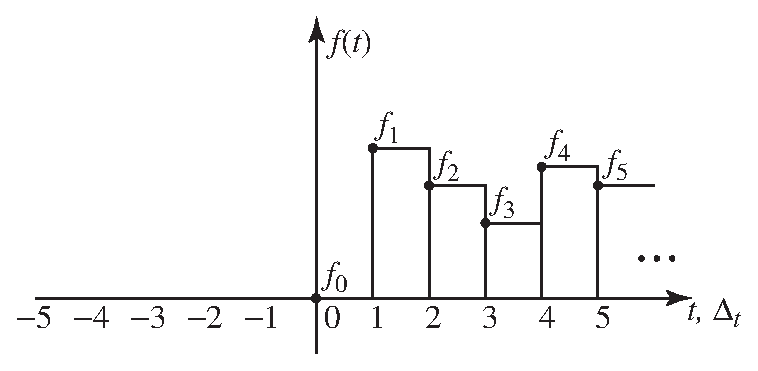
\epsfig{width=3.5in,file=Figures/Fdtd-pml/step-wise-function.eps} \\
  (a)\\
  \vspace{.15in}
  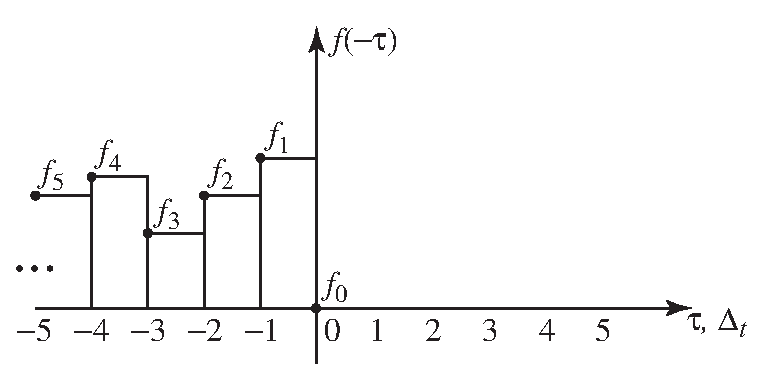
\epsfig{width=3.5in,file=Figures/Fdtd-pml/step-wise-reverse.eps}\\
  (b) \\
  \vspace{.15in}
  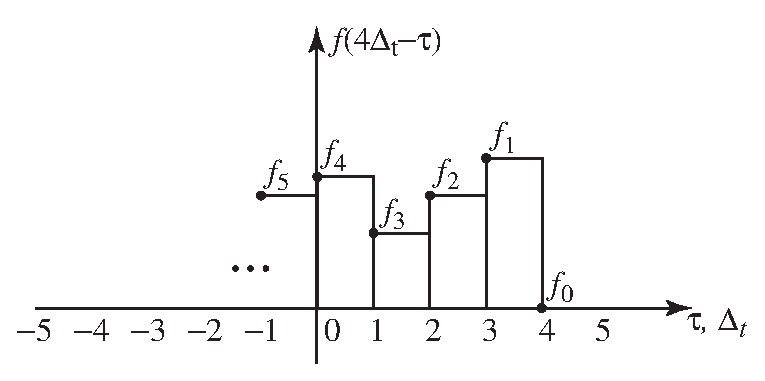
\epsfig{width=3.5in,file=Figures/Fdtd-pml/step-wise-reverse-shifted.eps}\\
  (c)
\mbox{}
\end{center} 
\caption{(a) Stepwise representation of a function
  $f(t)$.  The function is a constant $f_0$ for $0\leq t< \Delt$,
  $f_1$ for $\Delt \leq t< 2\Delt$, $f_2$ for $2 \Delt \leq t <
  3\Delt$, and so on. (b) Stepwise representation of a function
  $f(-\tau)$.  Here the constants $f_n$ are flipped about the origin
  but the pulses still extend for one time-step to the right of the
  corresponding point.  Hence the function is a constant $f_1$ for
  $-\Delt\leq\tau<0$, $f_2$ for $-2\Delt\leq\tau<-\Delt$, etc. (c)
  Stepwise representation of the function $f(q\Delt-\tau)$ when
  $q=4$.}  \label{fig:stepwise}
\end{figure}

The convolution contains the function $f(q\Delt-\tau)$.  At time-step
zero (i.e., $q=0$), this is merely $f(-\tau)$ which is illustrated in
Fig.\ \ref{fig:stepwise}(b).  Here all the sample points $f_n$ are
flipped symmetrically about the origin.  We assume that the function
is constant to the right of these sample points so that the function
is $f_1$ for $-\Delt\leq\tau<0$, it is $f_2$ for
$-2\Delt\leq\tau<-\Delta$, $f_3$ for $-3\Delt\leq\tau<-2\Delt$, and so
on.

Fig.\ \ref{fig:stepwise}(c) shows an example of $f(q\Delt-\tau)$ when
$q\neq 0$, specifically for $q=4$.  Recall that in
\refeq{eq:psiFunction} the limits of integration are from zero to
$q\Delt$---we do not need to concern ourselves with $\tau$ less than
zero nor greater than $q\Delt$.  As shown in Fig.\
\ref{fig:stepwise}(c), the first ``pulse'' extending to the right of
$\tau=0$ has a value of $f_q$, the pulse extending to the right of
$\tau=\Delt$ has a value of $f_{q-1}$, the one to the right of
$\tau=2\Delt$ has a value of $f_{q-2}$, and so on.  Thus, this shifted
function can be written as
\begin{equation}
  f(q\Delt-\tau) = \sum_{i=0}^{q-1}f_{q-i}p_i(\tau).
\end{equation}
Returning to the derivative of the magnetic field, we write
\begin{equation}
  \frac{\partial H_v(q\Delt-\tau)}{\partial w} = 
  \sum_{i=0}^{q-1}\frac{\partial H_v^{q-i}}{\partial w}p_i(\tau)
\end{equation}
where $H_v^{q-i}$ is the magnetic field at time-step $q-i$ and, when
implemented in the FDTD algorithm, the spatial derivative will be
realized as a spatial finite difference.

At time-step $q$, $\Psi_{E_uw}$ is given by
\begin{equation}
  \Psi_{E_uw}^q =
  \int_{\tau=0}^{q\Delt} \zeta_w(\tau) 
   \sum_{i=0}^{q-1} \frac{\partial H_v^{q-i}}{\partial w}p_i(\tau) d\tau
\end{equation}
Interchanging the order of summation and integration yields
\begin{eqnarray}
  \Psi_{E_uw}^q &=&
     \sum_{i=0}^{q-1} \frac{\partial H_v^{q-i}}{\partial w}
     \int_{\tau=0}^{q\Delt} \zeta_w(\tau)p_i(\tau) d\tau, 
     \label{eq:psiIntOne}
  \\
   &=&
     \sum_{i=0}^{q-1} \frac{\partial H_v^{q-i}}{\partial w}
     \int_{\tau=i\Delt}^{(i+1)\Delt} \zeta_w(\tau) d\tau,
     \label{eq:psiIntTwo}
\end{eqnarray}
where, in going from \refeq{eq:psiIntOne} to \refeq{eq:psiIntTwo}, the
pulse function was used to establish the limits of integration.

Consider the following integral
\begin{eqnarray}
  -\int_{i\Delta}^{(i+1)\Delta} e^{-a t}dt &=&
     \left. \frac{1}{a} e^{-at} \right|_{i\Delta}^{(i+1)\Delta}\\
   &=& \frac{1}{a} \left(e^{-a(i+1)\Delta} - e^{-ai\Delta}\right) \\
   &=& \frac{1}{a} \left(e^{-a\Delta}-1\right)e^{-ai\Delta} \\
   &=& \frac{1}{a} \left(e^{-a\Delta}-1\right)
                   \left(e^{-a\Delta}\right)^i
\end{eqnarray}
Keeping this in mind, the integration in \refeq{eq:psiIntTwo} can be
written as
\begin{eqnarray}
  \int_{\tau=i\Delt}^{(i+1)\Delt} \zeta_w(\tau) d\tau &=&
  -\frac{\sigma_w}{\kappa_w^2\epsilon_0}
  \int_{\tau=i\Delt}^{(i+1)\Delt}
   \exp\!\left(-\tau\left[\frac{a_w}{\epsilon_0}+
                       \frac{\sigma_w}{\kappa_w\epsilon_0}\right]\right)
    d\tau \\
  &=& C_w (b_w)^i
  \label{eq:cbTerm}
\end{eqnarray}
where
\begin{eqnarray}
  b_w &=& \exp\!\left(-\left[
    \frac{a_w}{\epsilon_0} +
    \frac{\sigma_w}{\kappa_w\epsilon_0}\right]\Delt\right), \\
  C_w &=& \frac{\sigma_w}{\sigma_w\kappa_w + \kappa_w^2 a_w}
          \left(b_w - 1\right).
\end{eqnarray}
Note that in \refeq{eq:cbTerm} $b_w$ is raised to the power $i$ which
is an integer index.  It is now possible to express $\Psi_{E_uw}^q$ as
\begin{equation}
  \Psi_{E_uw}^q =
  \sum_{i=0}^{q-1} \frac{\partial H_v^{q-i}}{\partial w} C_w (b_w)^i.
  \label{eq:psiSum}
\end{equation}
Let us explicitly separate the $i=0$ term from the rest of the
summation: 
\begin{equation}
  \Psi_{E_uw}^q =
   C_w \frac{\partial H_v^q}{\partial w}+ 
  \sum_{i=1}^{q-1} \frac{\partial H_v^{q-i}}{\partial w} C_w (b_w)^i.
\end{equation}
Replacing the index $i$ with $i'=i-1$ (so that $i=i'+1$), this becomes
\begin{equation}
  \Psi_{E_uw}^q =
   C_w \frac{\partial H_v^q}{\partial w}+ 
  \sum_{i'=0}^{q-2} 
    \frac{\partial H_v^{q-i'-1}}{\partial w} C_w (b_w)^{i'+1}.
\end{equation}
Dropping the prime from the index and rearranging slightly yields
\begin{equation}
  \Psi_{E_uw}^q =
  C_w \frac{\partial H_v^q}{\partial w}+ 
  b_w \sum_{i=0}^{[q-1]-1} 
    \frac{\partial H_v^{[q-1]-i}}{\partial w} C_w (b_w)^i.
\end{equation}
Comparing the summation in this expression to the one in
\refeq{eq:psiSum} one sees that this expression can be written as
\begin{equation}
  \Psi_{E_uw}^q =
  C_w \frac{\partial H_v^q}{\partial w} + 
  b_w \Psi_{E_uw}^{q-1}.
  \label{eq:psiRecursive}
\end{equation}
Note that $\Psi_{E_uw}$ at time-step $q$ is a function of
$\Psi_{E_uw}$ at time-step $q-1$.  Thus $\Psi_{E_uw}$ can be
updated recursively---there is no need to store the entire history of
$\Psi_{E_uw}$ to obtain the next value.  As is typical with FDTD, one
merely needs to know $\Psi_{E_uw}$ at the previous time step.

We now have all the pieces in place to implement a PML in the FDTD
method.  The algorithm to update the electric fields is
\begin{enumerate}
\item Update the $\Psi_{E_uw}$ terms employing the recursive update
equation given by \refeq{eq:psiRecursive}.  Recall that these 
$\Psi_{E_uw}$ functions represent the convolutions given in the second
line of \refeq{eq:exInPml}.
\item Update the electric fields in the standard way.  However, 
incorporate the $\kappa$'s where appropriate.  Essentially one
employs the update equation implied by the top line of
\refeq{eq:exInPml} (where that equation applies to $E_x$ and similar
equations apply to $E_y$ and $E_z$).  
\item Apply, i.e., add or subtract, $\Psi_{E_uw}$ to the electric
field as indicated by the second line of \refeq{eq:exInPml}.
\end{enumerate}
This completes the update of the electric field.

The magnetic fields are updated in a completely analogous manner.
First the $\Psi$ functions that pertain to the magnetic fields are
updated (in this case there are $\Psi_{H_uw}$ functions that involve
the spatial derivatives of the electric fields), then the magnetic
fields are updated in the usual way (accounting for any $\kappa$'s),
and finally the $\Psi$ functions are applied to the magnetic fields
(i.e., added or subtracted).
